\documentclass[UTF8,a4paper,12pt]{ctexbook} 

\usepackage{graphicx}%学习插入图
\usepackage{verbatim}%学习注释多行
\usepackage{booktabs}%表格
\usepackage{geometry}%图片
\usepackage{amsmath}
\usepackage{amssymb}
\usepackage{listings}%代码
\usepackage{xcolor}  %颜色
\usepackage{enumitem}%列表格式
\setenumerate[1]{itemsep=0pt,partopsep=0pt,parsep=\parskip,topsep=5pt}
\setitemize[1]{itemsep=0pt,partopsep=0pt,parsep=\parskip,topsep=5pt}
\setdescription{itemsep=0pt,partopsep=0pt,parsep=\parskip,topsep=5pt}
\usepackage{tcolorbox}
\usepackage{algorithm}  %format of the algorithm
\usepackage{algorithmic}%format of the algorithm
\usepackage{multirow}   %multirow for format of table
\usepackage{tabularx} 	%表格排版格式控制
\usepackage{array}	%表格排版格式控制
\usepackage{hyperref} %超链接 \url{URL}
\usepackage{tikz}
\usepackage{dirtree}

\CTEXsetup[format+={\flushleft}]{section}

%%%% 设置图片目录
\graphicspath{{figure/}}

%%%% 段落首行缩进两个字 %%%%
\makeatletter
\let\@afterindentfalse\@afterindenttrue
\@afterindenttrue
\makeatother
\setlength{\parindent}{2em}  %中文缩进两个汉字位

%%%% 下面的命令重定义页面边距,使其符合中文刊物习惯 %%%%
\addtolength{\topmargin}{-54pt}
\setlength{\oddsidemargin}{0.63cm}  % 3.17cm - 1 inch
\setlength{\evensidemargin}{\oddsidemargin}
\setlength{\textwidth}{14.66cm}
\setlength{\textheight}{24.00cm}    % 24.62

%%%% 下面的命令设置行间距与段落间距 %%%%
\linespread{1.4}
\setlength{\parskip}{0.5\baselineskip}
\geometry{left=1.6cm,right=1.8cm,top=2cm,bottom=1.7cm} %设置文章宽度
\pagestyle{plain} 		  %设置页面布局

%代码效果定义
\definecolor{mygreen}{rgb}{0,0.6,0}
\definecolor{mygray}{rgb}{0.5,0.5,0.5}
\definecolor{mymauve}{rgb}{0.58,0,0.82}
\lstset{ %
	backgroundcolor=\color{white},   % choose the background color
	basicstyle=\footnotesize\ttfamily,      % size of fonts used for the code
	%stringstyle=\color{codepurple},
	%basicstyle=\footnotesize,
	%breakatwhitespace=false,         
	%breaklines=true,                 
	%captionpos=b,                    
	%keepspaces=true,                 
	%numbers=left,                    
	%numbersep=5pt,                  
	%showspaces=false,                
	%showstringspaces=false,
	%showtabs=false,        
	columns=fullflexible,
	breaklines=true,                 % automatic line breaking only at whitespace
	captionpos=b,                    % sets the caption-position to bottom
	tabsize=4,
	commentstyle=\color{mygreen},    % comment style
	escapeinside={\%*}{*)},          % if you want to add LaTeX within your code
	keywordstyle=\color{blue},       % keyword style
	stringstyle=\color{mymauve}\ttfamily,     % string literal style
	frame=single,
	rulesepcolor=\color{red!20!green!20!blue!20},
	% identifierstyle=\color{red},
	language=c++,
}
 \author{\kaishu 郑华}
 \title{\heiti 音乐笔记}
 
\begin{document}          %正文排版开始
 	\maketitle
 
\chapter{看谱唱歌、乐理基础}
	\section{音名、唱名、音符、休止符、拍号}
	 	常用符号表示记号:\url{https://blog.csdn.net/chuchus/article/details/46042673}
	 	
		\subsection*{唱名}
		 	
		 	\verb|do(1)  re(2)  mi(3)  fa(4)  sol(5)  la(6)  si(7)| 
		 
		\subsection*{音名}
		 	
		 	\verb|C       D       E      F       G      A      B|
	 
		\subsection*{音符、休止符}
			
			全音符、  2分、  4分、   8分、  16分、  32分。具体的是1对2的关系,一个全音符等于两个2分音符,以此类推。
		
			\begin{figure}[H]
				\centering
				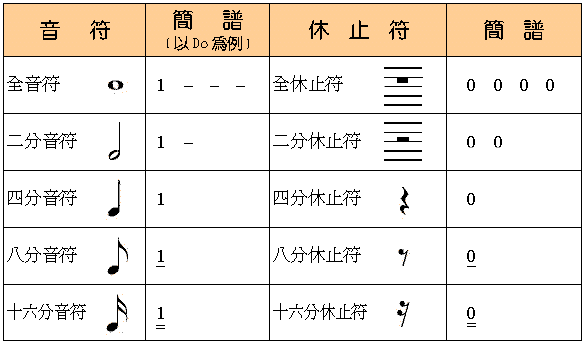
\includegraphics[scale=0.7]{yinfu}
				\caption{音符与休止符表示记号}
			\end{figure}
			
		\subsection*{拍号(拍子记号)}
			$\dfrac{\textbf{每小节有几拍}}{\textbf{x分音符当1拍}} $,如$\dfrac{3}{4} $(每小节有3拍,每个4分音符当一拍)、  $\dfrac{2}{2} $ (每小节有2拍,每个2分音符当一拍)等.
			
		\subsection{半音}
			只有 3-4,7-$\hat{1}$ 是半音。
			
			对应于钢琴上的相邻键。
			
			对应于吉他上的相邻品。
			
			\begin{figure}[H]
				\centering
				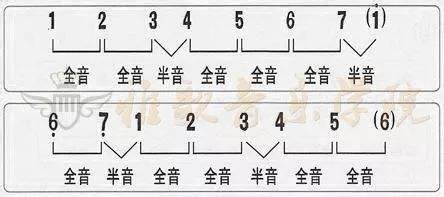
\includegraphics[width=12cm,height=4cm]{timg.jpg}
				\caption{全音半音演示}
			\end{figure}
			
		\subsection{反复记号,附点音符}
			\begin{figure}[H]
				\centering
				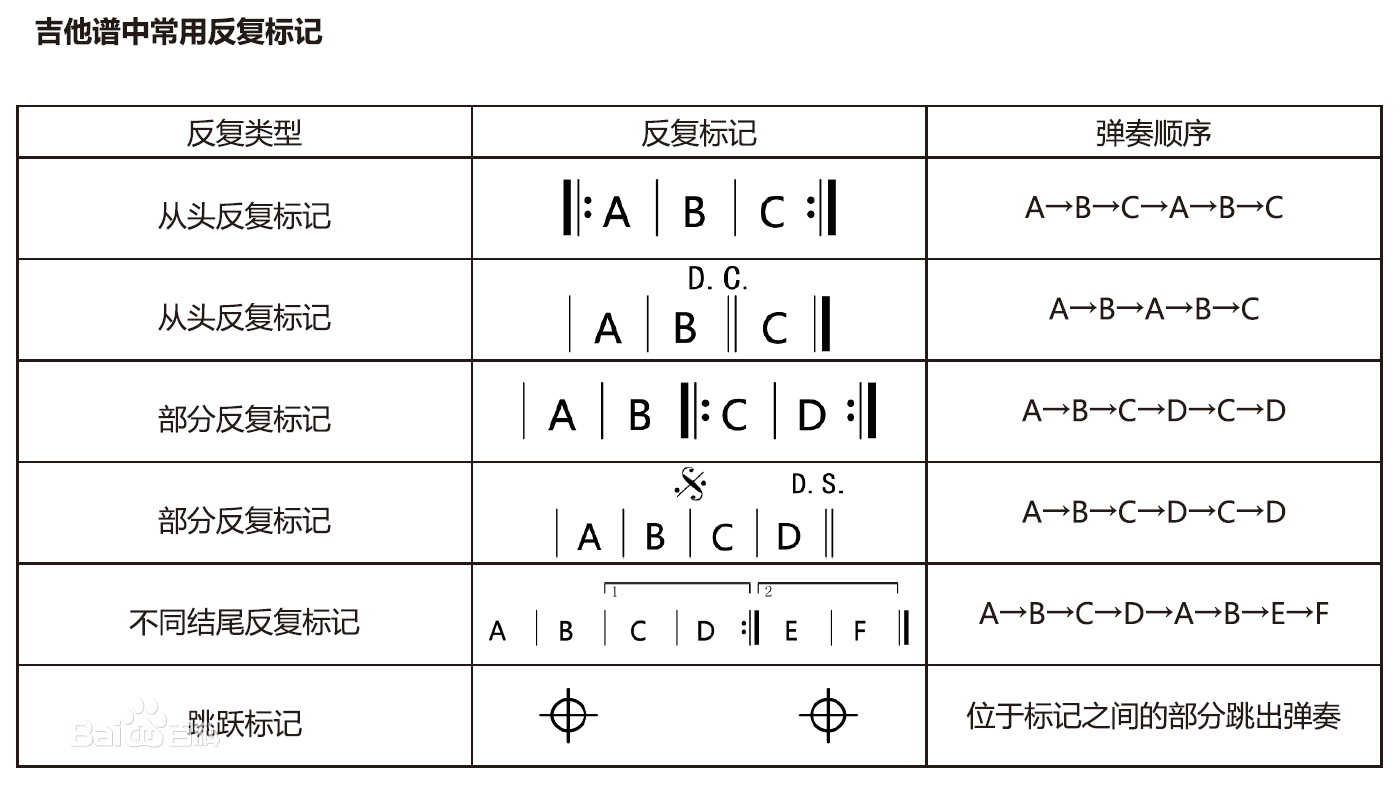
\includegraphics[scale=0.34]{repeat}
				\caption{重复标记}
			\end{figure}
		\subsection{音程}
			用“度”来表示。
			\paragraph{小2度 -基础}
				小二度也被称为\textbf{半音}。 也是吉他最小的音程单位。
				
				就是同一根琴弦上\textbf{相邻(挨着)的两个品}之间。
				
			\paragraph{大2度 -基础}
				大2度也被称为\textbf{全音}。
				
				在吉他上就是同一根琴弦上\textbf{相隔1品},如1品与3品等。
				
				不同的弦则表现为,\underline{6-5-4-3弦,2-1弦} \textbf{3品到下根弦}为全音, 而 \underline{3-2弦} 则是\textbf{2品到下根弦}为全音。
				
			\paragraph{小3度 -重点}
				包含一个全音和半音,就是一个\textbf{全音+半音=小三度}。
				
				在吉他上,就是\textbf{同一根弦上相隔3品},如1品与4品。

				不同的弦则表现为,\underline{6-5-4-3弦,2-1弦} \textbf{2品到下根弦}为全音, 而 \underline{3-2弦} 则是\textbf{1品到下根弦}为全音。
				
			\paragraph{大3度 -重点}		
				包含两个全音,就是 \textbf{全音+全音=大三度},如1-3
				
				在吉他上,就是\textbf{同一根弦上相隔4品},如1品与5品。\textit{(相隔2个品,中间又存一个品,再加1个要按的品)}
				
				不同的弦则表现为,\underline{6-5-4-3弦,2-1弦} \textbf{1品到下根弦}为全音, 而 \underline{3-2弦} 则是\textbf{直接到下根弦}为全音。
			\paragraph{纯4度}
				包含两个全音和一个半音,就是\textbf{全音+全音+半音 = 纯四度},如1-4
				
				在吉他上,就是\textbf{同一根弦上相隔5品},如1品与6品。
				
				不同的弦则表现为,\textbf{相邻两个弦上相同的两个品}。
				
			\paragraph{增4度  \&  减5度}				
				继续增加一个半音,就是\textbf{3个全音=增四度},\verb|1-#4|
				
			\paragraph{纯5度}				
				继续增加一个半音,就是\textbf{3个全音+半音=纯5度},如1-5, 2-6
				
			\paragraph{小6度}
				继续增加一个半音,就是\textbf{4个全音=小六度}, 如1-b6
				
			\paragraph{大6度}	
				继续增加一个半音,就是\textbf{4个全音 + 半音 =大六度},  如1-6
				
			\paragraph{小7度}
				继续增加一个半音,就是\textbf{5个全音=小七度},如1-b7
				
			\paragraph{大7度}	
				继续增加一个半音,就是\textbf{5个全音+ 半音=大七度},如1-7
				
			\paragraph{纯8度}	
				继续增加一个半音,就是\textbf{6个全音= 八度},如1-$\hat{1}$
							
\chapter{钢琴-简谱与五线谱的弹奏}

\chapter{作曲及和弦}
	\section{和弦}
		\subsection{构成和性质}
			是由两个或两个以上的音叠加而成的。
			
		\subsection{大三和弦}
			$$ \textbf{根音 + 大三度 + 小三度} $$
			
			\underline{1 大三度 3  小三度 5}, \textbf{根音1}的\textbf{音名为C}, 所以这个大三和弦叫\textbf{C和弦}。

			\underline{5 大三度 7  小三度 2}, \textbf{根音5}的\textbf{音名为G}, 所以这个大三和弦叫\textbf{G和弦}。
			
		\subsection{小三和弦}
			$$ \textbf{根音 +  小三度 + 大三度} $$
	
			\underline{6 小三度 1  大三度 3}, \textbf{根音6}的\textbf{音名为A},\textit{小三和弦需加脚码}$_m$,所以这个叫\textbf{$\mathbf{A_m}$和弦}。
			
			\underline{3 小三度 5  大三度 7}, \textbf{根音3}的\textbf{音名为E},\textit{小三和弦需加脚码}$_m$,所以这个叫\textbf{$\mathbf{E_m}$和弦}。
		
		
		\subsection{七和弦}
		
		\subsection{五和弦}
			
		\subsection{扫弦}
			和弦外音不能扫。
			
			节奏、强弱、准确
			
		\subsection{击弦}
		
		\subsection{琶音}
		
		\subsection{右手切音}
		
		
\chapter{和声与编曲}

\chapter{吉他入门}
		    
\end{document} 